% Commands
% Document class
\documentclass[a4paper, 11pt]{report}
\usepackage[utf8]{inputenc}

% Table of contents
\usepackage[nottoc,notlof,notlot]{tocbibind} % including references
\setcounter{tocdepth}{2} % depth
\setcounter{secnumdepth}{3} % section numbering depth

% Miscellaneous
\usepackage{fullpage} % different margins
\usepackage{hyperref} % links
\usepackage[binary-units=true]{siunitx} % MB, GB, etc.
\usepackage{pdfpages} % import PDFs
\usepackage{verbatim} % multi-line comments

% Checkmarks and xmarks
\usepackage{amssymb}
\usepackage{pifont}
\definecolor{green}{RGB}{0,176,80}
\newcommand{\cmark}{{\color{green}\textbf{\ding{51}}} }
\definecolor{red}{RGB}{222,0,0}
\newcommand{\xmark}{{\color{red}\textbf{\ding{55}}} }

% Adding a dot at the end of paragraph titles
\let\originalparagraph\paragraph
\renewcommand{\paragraph}[2][.]{\originalparagraph{#2#1}}

% Glossaries and acronyms
% section,numberedsection=autolabel
\usepackage[acronym,toc]{glossaries} % package
% General
\newacronym{rm}{RM}{Resource Manager}
\newacronym{rmf}{RMF}{Resource Management Framework}
\newacronym{vm}{VM}{Virtual Machine}
\newacronym{inp}{INP}{In-Network Processing}
\newacronym{nfv}{NFV}{Network Function Virtualization}
\newacronym{sdn}{SDN}{Software Defined Networking}
\newacronym{tor}{ToR}{Top of Rack}
\newacronym{hpc}{HPC}{High Performance Computing}
\newacronym{dht}{DHT}{Distributed hash table}

% Programming
\newacronym{api}{API}{Application Programming Interface}
\newacronym{mpi}{MPI}{Message Passing Interface}
\newacronym{rpc}{RPC}{Remote Procedure Call}

% Resource models
\newacronym{vc}{VC}{Virtual Cluster}
\newacronym{voc}{VOC}{Virtual Oversubscribed Cluster}
\newacronym{tivc}{TIVC}{Time-Interleaved Virtual Cluster}
\newacronym{tag}{TAG}{Tenant Application Graph}

% SHArP
\newacronym{an}{AN}{Aggregation Node}
\newacronym{am}{AM}{Aggregation Manager}
\newacronym{tca}{TCA}{Target Channel Adapter}
\newacronym{qp}{QP}{Queue Pair}
\newglossaryentry{ibm}{
    name=IBM,
    description=IBM\textsuperscript{\textregistered}
}
\newglossaryentry{switchib2}{
    name=Mellanox's SwitchIB-2,
    description=Mellanox's SwitchIB-2\textsuperscript{TM}
}

% Apache Hadoop YARN
\newglossaryentry{apache}{
    name=Apache,
    description=Apache\textsuperscript{TM}
}
\newglossaryentry{hadoop}{
    name=Apache Hadoop,
    description=\glsdesc{apache} Hadoop\textsuperscript{\textcopyright}
}
\newglossaryentry{yarn_full}{
    name=Apache Hadoop YARN,
    description=\glsdesc{hadoop} YARN \texorpdfstring{\cite{yarn}}{}
}
\newglossaryentry{yarn}{
    name=Apache YARN,
    description=\glsdesc{apache} YARN \texorpdfstring{\cite{yarn}}{}
} % acronyms
% Glossary definition
\newglossary*{resources}{Resources glossary}

\newglossaryentry{resource:physical}{
    type=resources,
    name=Physical resource,
    text=physical resource,
    description={physical hardware component of limited availability within a physical machine}
}

    \newglossaryentry{resource:physical:server}{
        type=resources,
        name=Physical server resource,
        text=physical server resource,
        parent=resource:physical,
        description={resource of a physical server machine}
    }
    
    \newglossaryentry{resource:physical:switch}{
        type=resources,
        name=Physical switch resources,
        text=physical switch resources,
        parent=resource:physical,
        description={resource of a physical switche, network accelerator, middle-box and of every kind of network device originally intended to forward packets}
    }
    
\newglossaryentry{resource:logical}{
    type=resources,
    name=Logical resource,
    text=logical resource,
    description={logical representation of a physical resource}
}

    \newglossaryentry{resource:logical:server}{
        type=resources,
        name=Logical server resource,
        text=logical server resource,
        parent=resource:logical,
        description={virtualized server physical resource, often implemented by means of a \gls{vm}, container or an entire physical server}
    }
    
    \newglossaryentry{resource:logical:switch}{
        type=resources,
        name=Logical switch resource,
        text=logical switch resource,
        parent=resource:logical,
        description={logical representation of a physical switch resource not mapped to any physical switch device}
    }
    
    \newglossaryentry{resource:logical:edge}{
        type=resources,
        name=Logical edge resource,
        text=logical edge resource,
        parent=resource:logical,
        description={properties of virtual connections between two logical resources, e.g., bandwidth, latency, etc}
    }
    
\newglossaryentry{resource:composite}{
    type=resources,
    name=Composite,
    text=composite,
    description={template describing a high-level logical component.
        It can be made out of other composites and/or logical resources.}
}

    \newglossaryentry{resource:composite:server}{
        type=resources,
        name=Server composite,
        text=server composite,
        parent=resource:composite,
        description={composite describing a high-level server component, e.g., \textit{web server}, \textit{databases}, etc}
    }
    
    \newglossaryentry{resource:composite:inp}{
        type=resources,
        name=\gls{inp} composite,
        text=\texorpdfstring{\gls{inp}}{INP} composite,
        parent=resource:composite,
        description={composite describing a high-level \gls{inp} application, e.g., \textit{IncBricks} \cite{incbricks}, \textit{NetChain} \cite{netchain}, etc}
    }
    
\newglossaryentry{model}{
    type=resources,
    name=Resource model,
    text=resource model,
    description={model capable of describing composites and logical resources.
        The model exposed to tenants and the one internally used by the \gls{rm} could be different}
}

    \newglossaryentry{model:tenant}{
        type=resources,
        name=Tenant-side model,
        text=tenant-side model,
        parent=model,
        description={resource model exposed to tenants by the system \gls{api}}
    }
    
    \newglossaryentry{model:rm}{
        type=resources,
        name=\gls{rm}-side model,
        text=\texorpdfstring{\gls{rm}}{RM}-side model,
        parent=model,
        description={resource model internally used by the placement algorithm in order to allocate logical resources}
    } % resources glossary
\makeglossaries % computing the glossary and acronyms list

% In-line lists
\usepackage[inline]{enumitem}
\newlist{mylist}{enumerate*}{1}
\setlist[mylist]{label=(\roman*)}

% References sections
\renewcommand{\sectionautorefname}{\S}
\renewcommand{\subsectionautorefname}{\S}
\renewcommand{\subsubsectionautorefname}{\S}
\renewcommand\bibname{References}

% Capitalized references
\usepackage{cleveref}

% Footnotes with symbols
\usepackage[symbol]{footmisc}
\renewcommand{\thefootnote}{\fnsymbol{footnote}}

\title{Data center resource management for in-network processing}
% \subtitle{A modern beamer theme}
\date{} % FIXME
\author{Marco Micera}
\institute{Politecnico di Torino, Technische Universit{\"a}t Darmstadt}
% \titlegraphic{\hfill\includegraphics[height=1.5cm]{logo.pdf}}

\begin{document}

\maketitle

\begin{frame}{Outline}
  \setbeamertemplate{section in toc}[sections numbered]
  \tableofcontents[hideallsubsections]
\end{frame}

\section{Introduction}

\begin{frame}[fragile]{Introduction}
  \begin{itemize}
    \item (NetCache introduction: "modern Internet services, such as search, social networking and e-commerce, critically depend on high-performance key-value stores. Rendering even a single web page often requires hundreds or even thousands of storage accesses." \cite{netchain}
    \item need to scale up (SHArP introduction, \textit{justifying INP}: "As the number of compute elements grows, and the need to expose and utilize higher levels of parallelism grows, it is essential to reconsider system architectures, and focus on developing architectures that lend themselves better to providing extreme-scale simulation capabilities.") \cite{sharp}
    \item However, modern-day data centers only exploit servers to perform computation % FIXME
  \end{itemize}

\end{frame}
\begin{frame}[fragile]{In-Network Processing (INP)}
  \begin{itemize}
    \item Offloading computation to network devices (e.g., programmable switches, network accelerators, middleboxes, etc.), hence reducing load on servers
    \item (Daiet introduction: "The functionality of networks can now be enriched without hardware changes while retaining the capability of processing packets at very high rates, even above Terabits per second") \cite{daiet}
    \item Few solutions out there already: Daiet \cite{daiet}, SHArP \cite{sharp}, NetChain \cite{netchain}, IncBricks \cite{incbricks}
  \end{itemize}
\end{frame}
\begin{frame}[fragile]{Problem statement}
  \begin{itemize}
    \item TODO mention network-aware RMs % TODO
    \item there is no \gls{rm} that considering server and switch resources \textbf{conjunctly}...
  \end{itemize}
\end{frame}
\begin{frame}[fragile]{Goals}
  (abstract)
  \begin{enumerate}
    \item Model and evaluate an API through which applications can ask for INP resources
    \item Discuss the importance of a scheduler which can reject INP requests and propose their server-only equivalent when needed (e.g., high switch utilization)
  \end{enumerate}
\end{frame}

\section{Analysis}

\begin{frame}{Currently existing \gls{inp} solutions}
  \begin{itemize}
    \item In-network \textbf{storage}
    \begin{itemize}
      \item Switches must
      \begin{itemize}
        \item dedicate part of their local memory to store a distributed map
        \item form a chain
      \end{itemize}
      \item IncBricks \cite{incbricks}, NetChain \cite{netchain}
    \end{itemize}
		\item In-network \textbf{data aggregation}
    \begin{itemize}
      \item Switches must
      \begin{itemize}
        \item form a tree whose root is connected to data consumers and whose leaves are connected to data producers
        \item dedicate part of their local memory to store a key-value map
        \item be able to perform basic operations on data, such as writing and hashing
        \item wait for all its children to send aggregated data
      \end{itemize}
      \item Daiet \cite{daiet}, SHArP \cite{sharp}
    \end{itemize}
	\end{itemize}
\end{frame}
\begin{frame}{In-network caching system: IncBricks}
  % \begin{itemize}
  %   \item Custom fabric \textit{IncBox} (programmable switch + network accelerator)
  % \end{itemize}
  \centering
  \includegraphics[page=1, clip, trim=3.6cm 0.7cm 2.5cm 3.75cm, width=\textwidth]{analysis/inp/solutions.pdf}
\end{frame}
\begin{frame}{In-network caching system: IncBricks}
  \centering
  \includegraphics[page=2, clip, trim=3.6cm 0.7cm 2.5cm 3.75cm, width=\textwidth]{analysis/inp/solutions.pdf}
\end{frame}
\begin{frame}{In-network caching system: IncBricks}
  \centering
  \includegraphics[page=3, clip, trim=3.6cm 0.7cm 2.5cm 3.75cm, width=\textwidth]{analysis/inp/solutions.pdf}
\end{frame}
\begin{frame}{Coordination services: NetChain}
  \centering
  \includegraphics[page=6, clip, trim=3.6cm 0.7cm 3.2cm 4cm, width=\textwidth]{analysis/inp/solutions.pdf}
\end{frame}
\begin{frame}{In-network aggregation: Daiet}
  % Daiet \cite{daiet} is a system that performs in-network data aggregation for partition\hyp{}aggregate data center applications (big data analysis such as MapReduce \cite{mapreduce}, machine learning, graph processing, and stream processing). Inventors claim to achieve an 86.9\%-89.3\% traffic reduction, causing the execution time at the reducer to drop by 83.6\% on average.
  \centering
  \includegraphics[page=10, clip, trim=0.5cm 0.7cm 1.2cm 2.6cm, width=\textwidth]{analysis/inp/solutions.pdf}
\end{frame}
\begin{frame}{In-network aggregation: Daiet}
  \centering
  \includegraphics[page=11, clip, trim=0.35cm 0.6cm 0.3cm 2.6cm, width=\textwidth]{analysis/inp/solutions.pdf}
\end{frame}
\begin{frame}{Aggregation protocol: SHArP}
  \centering
  \includegraphics[page=15, clip, trim=3.3cm 0.9cm 1.6cm 3.4cm, width=\textwidth]{analysis/inp/solutions.pdf}
\end{frame}
\begin{frame}{Resource models (3.4)}
  \begin{columns}[T,onlytextwidth]
    \column{0.4\textwidth}
      \begin{enumerate}
        \item \glsentryfull{vc}\\
        \begin{center}
          \includegraphics[page=1, clip, trim=0.5cm 0.6cm 3.85cm 1cm, width=0.7\textwidth]{analysis/models/solutions.pdf}
        \end{center}
        \item \glsentryfull{voc}
        \begin{itemize}
          \item $N$ \glsentryshortpl{vc} connected to a single root virtual switch
        \end{itemize}
        % \begin{center}
        %   \includegraphics[page=2, clip, trim=0.5cm 0.6cm 0.5cm 0.7cm, width=\textwidth]{analysis/models/solutions.pdf}
        % \end{center}
      \end{enumerate}
    \column{0.6\textwidth}
      \begin{enumerate}
        \setcounter{enumi}{2}
        \item \glsentryfull{tag}\\
        \begin{center}
          \includegraphics[page=3, clip, trim=0.5cm 0.5cm 0.5cm 0.5cm, width=0.95\textwidth]{analysis/models/solutions.pdf}
        \end{center}
        \item Fine-grained resource requests
        \begin{itemize}
          \item List of server-only resource demands
        \end{itemize}
        \item High-level goals
        \begin{itemize}
          \item E.g., job completion time (Bazaar \cite{bazaar})
        \end{itemize}
      \end{enumerate}
  \end{columns}
\end{frame}
\begin{frame}{Intregrating INP resources in RMs}
  (3.3)
\end{frame}
\begin{frame}{Level of network awareness in RMs}
  % 3.3.2
  \vspace{2mm}
  \begin{itemize}
    \item \glsentryshortpl{vm} proximity-aware
    \begin{itemize}
      \item Spreading \glsentryshortpl{vm} across different failure domains (e.g., racks, power domains, etc.)
      \item Omega \cite{omega}, \glsdesc{yarn}, Mesos \cite{mesos}, etc.
    \end{itemize}
    \item Bandwidth-aware
    \begin{itemize}
      \item Allowing tenants to specify bandwidth demands
      \item "Virtual network" models (i.e., \glsentryshortpl{vc}, \glsentryshortpl{voc} and \glsentryshortpl{tag})
      \item CloudMirror \cite{cloudmirror}, Oktopus \cite{oktopus}, Kraken \cite{kraken}, Proteus \cite{proteus}, etc.
    \end{itemize}
    \item Network resources-aware
    \begin{itemize}
      \item At the time of writing, there seemed to be only one embedding solution\footnote{\tiny{Rabbani, Md Golam, et al. "On tackling virtual data center embedding problem." \textit{2013 IFIP/IEEE International Symposium on Integrated Network Management (IM 2013)}. IEEE, 2013. \cite{ontackling}}} considering switch resources
      \item The scheduler places server and switch resources in separate rounds
    \end{itemize}
  \end{itemize}
  \vspace{5mm}
\end{frame}
% \begin{frame}{FIXME: the only “network-aware” RM + its problems}
%   (3.3.2)
% \end{frame}

% \section{Requirements} % FIXME Is this necessary?

\section{Design}
\begin{frame}{Composites}
  (Thesis repository \texttt{dock/thesis/figures/design/model/presentation.pdf})
\end{frame}
\begin{frame}{The extended-Tenant Application Graph (eTag)}
  \begin{itemize}
    \item (5.2.1 why existing resource models do not satisfy all requirements)
    \item (5.2.2 eTag)
  \end{itemize}
\end{frame}
\begin{frame}{The template database}
  \begin{itemize}
    \item (5.3 generic groups)
    \item (5.1.2 template database role)(5.1.2 template database role)
  \end{itemize}
\end{frame}
\begin{frame}{FIXME I should introduce composites earlier}
  % TODO I should mention generic groups
\end{frame}

\section{Conclusions}

% \begin{frame}{Summary}

%   Get the source of this theme and the demo presentation from

%   \begin{center}\url{github.com/matze/mtheme}\end{center}

%   The theme \emph{itself} is licensed under a
%   \href{http://creativecommons.org/licenses/by-sa/4.0/}{Creative Commons
%   Attribution-ShareAlike 4.0 International License}.

%   \begin{center}\ccbysa\end{center}

% \end{frame}

\begin{frame}[standout]
  Questions?
\end{frame}

\begin{frame}[standout]
  Thank you
\end{frame}

\appendix

% \begin{frame}[fragile]{Backup slides}
%   Sometimes, it is useful to add slides at the end of your presentation to
%   refer to during audience questions.

%   The best way to do this is to include the \verb|appendixnumberbeamer|
%   package in your preamble and call \verb|\appendix| before your backup slides.

%   \themename will automatically turn off slide numbering and progress bars for
%   slides in the appendix.
% \end{frame}

\begin{frame}[allowframebreaks]{Bibliography}
  \bibliographystyle{abbrv}
  \bibliography{../thesis/utility/references}
\end{frame}

\end{document}
